

\begin{center}
    {\bf КЛЮЧЕВАЯ ФУНКЦИЯ ДЛЯ УРАВНЕНИЯ БЕЛЕЦКОГО}

    {\it Т.И. Костина}

    (Воронеж; {\it tata@rambler.ru})
\end{center}

\addcontentsline{toc}{section}{Костина Т.И.}

	Математическая модель колебаний спутника в плоскости эллиптической орбиты, представленная уравнением Белецкого имеет следующий вид [1]:
 $$
(1+e\cos(\nu))\-
2e\sin(\nu)+\frac{d\delta}{d\nu}+\mu\sin(\delta)-4e\sin(\nu) =0,
\eqno{(1)}
 $$
где параметр $e$ --- эксцентриситет орбиты, $\mu$ --- параметр,
характеризующий распределение массы спутника, $\nu$ ---
угловая (полярная) координата центра масс спутника, $\delta$ --- угол
между фокальным радиусом и осью симметрии спутника.


В случаи  $e\neq0$ и  $\mu\neq1$ уравнение (3) не интегрируется, поэтому для его решения используются приближенные методы, например метод Ляпунова-Шмидта. Для его применения  было доказано  [3], что уравнение Белецкого является вариационным, был найден
интегрирующий множитель $(1+e\cos(\nu))$, при умножении на который уравнения (1) получается
 уравнением Эйлера-Лагранжа для экстремалей
функционала действия
 $$
V(q)=\int\limits_{0}^{2\pi}L(\dot{q},q)dt,
 $$
с лагранжианом $L(\dot{q},q)$:
 $$
\frac{\dot{q^2}}{2}(1+e\cos(\nu))^2+(1+e\cos(\nu))4eq\sin(\nu)+
(1+e\cos(\nu))\mu\cos(q).
 $$





 Затем ставится задача построения алгоритма получения и исследования ключевой функции. Приближенное построение
ключевых функций осуществляется на основе аппроксимации
Галеркина-Ритца и редукции Пуанкаре, с помощью численного метода градиентного спуска в точку минимума
функционала энергии $V$:
$$
 \frac 1{2\pi} \int\limits
_0^{2\pi}\left((1+\varepsilon\,e_1(t))^2 \ \frac{\dot{x}^2}{2} +
(1+\varepsilon\,e_1(t))( \mu
 \cos (x)+4\varepsilon x e_2(t))\right) dt.
 $$
 Получаются сходящиеся итерационные процессы, позволяющие строить ключевую функцию с  любой требуемой точностью.
$$
W(\xi_0, \xi_1, \xi_2,\mu,
\varepsilon)=\inf V (\xi_0 + \xi_1 e_{1} + \xi_2e_{2} +v),
 $$
 где $  e_{1}=\sqrt{2}\cos(t),  e_{2}=\sqrt{2}\sin(t).$

 В связи с развитием современной компьютерной техники и методов численного анализа стало возможным получить фазовые портреты решений и провести качественный анализ.
 При компьютерной реализации
вычисления и анализа  возникает существенные технические
трудности. Требуется наличие большого объёма оперативной памяти, иначе происходит зацикливание или зависание программ.
 Исследование облегчает наличие  круговой симметрии, возникающей из-за
того, что функционал действия инвариантен относительно
сдвига функции. Положив $\xi_2=0$ можно провести вторичную редукцию функционала.


Получены  компьютерные изображения поверхностей линий уровней
редуцированных приближений ключевой функции для уравнения Белецкого при двух различных значениях параметра:

\begin{center}
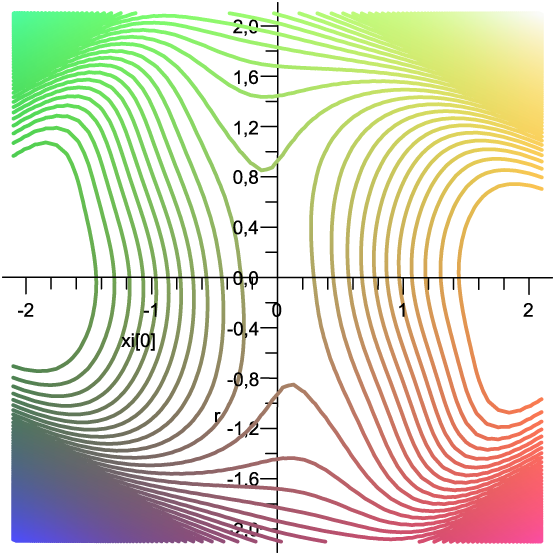
\includegraphics[width=0.3\textwidth,angle=0]{e01.png} \ \
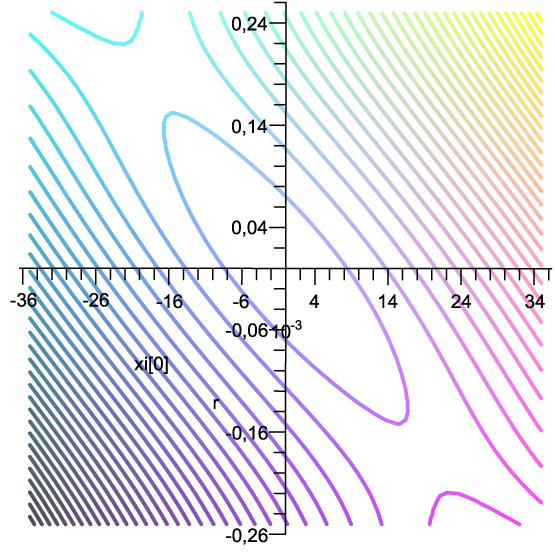
\includegraphics[width=0.3\textwidth,angle=0]{e02.png}

Рис. 1. Семейства линий уровней  ключевой функции  для уравнения Белецкого при {$\mu
= 1.1\,, \ \varepsilon=0.2\,;$ \ $\mu = 1.05\,, \
\varepsilon=0.1\,. $}

\end{center}

%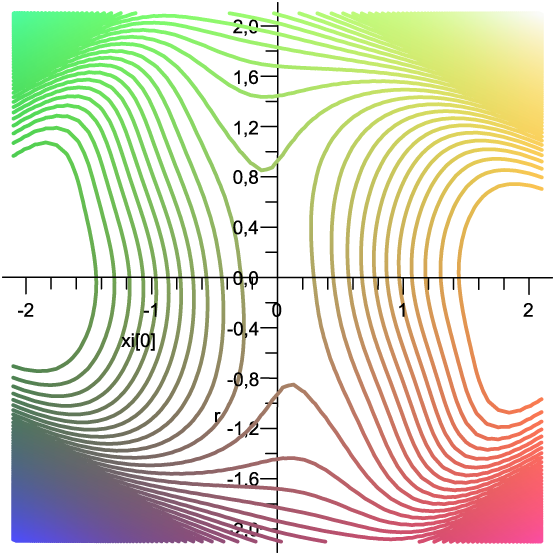
\includegraphics[width=0.3\textwidth,angle=0]{e01.eps} \ \
%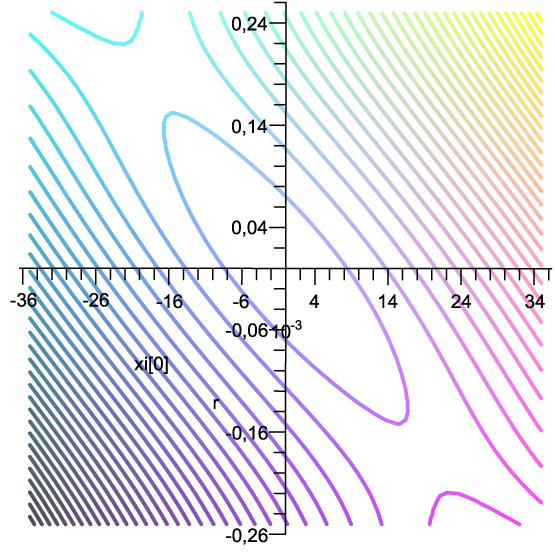
\includegraphics[width=0.3\textwidth,angle=0]{e02.eps}

%\includegraphics[width=0.3\textwidth,angle=0]{e01-d.eps} \ \
%\includegraphics[width=0.3\textwidth,angle=0]{e02-d.eps}

%\includegraphics[width=0.3\textwidth,angle=0]{e01-dd.eps} \ \
%\includegraphics[width=0.3\textwidth,angle=0]{e02-dd.eps}



% Оформление списка литературы
\smallskip \centerline {\bf Литература} \nopagebreak

1. Белецкий В.В. Движение искусственного спутника относительно центра масс.
-- М.: Наука, 1965. -- 416 с.


2. Костина Т.И. Нелокальное вычисление ключевых функций в задаче о
периодических решениях вариационных уравнений // Вестник
Воронежского государственного университета. Серия: Физика.
Математика. \No 1. 2011 -- С. 181-186.


3. Костина Т.И. О ветвлении периодических решений уравнения  колебаний маятника и уравнения Белецкого // Т.И. Костина, Ю.И. Сапронов // Вестник Воронежского Вестник
Воронежского государственного университета. Серия: Физика.
Математика. \No 1. 2018 -- С.99-114.



%\end{document} 